\NeedsTeXFormat{LaTeX2e}
\documentclass[12pt,a4paper,twoside]{scrartcl}
\usepackage{amsmath,amssymb,amsfonts,amscd}
\usepackage[amsthm,thmmarks]{ntheorem}
\usepackage{TheoremCollection}
\usepackage{accents}
\usepackage{bbm} % BlackBoeard letters
\usepackage{fancyheadings} %
\usepackage[small]{caption2} %
\usepackage{makeidx} %
\usepackage{fleqn} 
\usepackage{indentfirst} 
\usepackage{cancel} % \cancel{stuff} provides slashed stuff
\usepackage{graphicx} % \including PostScript
\usepackage{color}
\usepackage{pstricks}
\usepackage{pst-node,pst-plot}
\usepackage{nomencl} %Nomenklatur
\usepackage{mathrsfs}   % Schoenes Lagrange -L mit \mathscr{L}
\usepackage{pifont} % dinbgbats
\usepackage[small]{subfigure}
\usepackage{longtable}
\usepackage[plain]{fancyref}
\usepackage{cite}
%\usepackage[bbgreekl]{MyBbol}  % bb-Symbole auch griechisch
\usepackage[
        a4paper,      % A4
        dvips,        % Erzeugung durch dvips
        pdftitle={MixingParameterTools - Documentation}
	bookmarks=true,
	bookmarksnumbered=true, % Verwendete Bookmarks anzeigen
        colorlinks,   % Farbige Links
        linkcolor=blue,
        urlcolor=blue,
        citecolor=blue]{hyperref}
%\usepackage[dvips]{thumbpdf}

%-- page parameters -------------------------------------------------

\pagestyle{fancyplain}

\advance \headheight by 3.0truept       % for 12pt mandatory...
\lhead[\fancyplain{}{\thepage}]{\fancyplain{}{\rightmark}}
\rhead[\fancyplain{}{\leftmark}]{\fancyplain{\thepage}{\thepage}}
\cfoot{}

\addtolength{\oddsidemargin}{1.0truecm}
\addtolength{\evensidemargin}{-0.3truecm}

%-- end of page parameters ------------------------------------------


\makeindex
\makeglossary

% \newcommand{\WeightConnect}[4]{\ncline{->}{#1}{#2}\mput*{\ovalnode{#3}{#4}}
% \ncline{-}{#1}{#3}\ncline{->}{#3}{#2}}
% 
% \def\Nf{i}
% \def\Ng{j}
% \newcommand{\GroupIndex}[1]{\ifcase#1\or \or a\or b\or c\or d\or e\or f\or g\or h\or i\or j\or
% k\or l\or m\or n\or o\or p\or q\or r\or s\or t\or u\or v\or w\or x\or
% y\or z\else\@ctrerr\fi}
% \newcommand{\FamilyIndex}[1]{\ifcase#1\or \or f\or g\or h\or i\or j\or
% k\or l\or m\or n\or o\or p\or q\or r\or s\or t\or u\or v\or w\or x\or
% y\or z\else\@ctrerr\fi}
\def\chargec{\mathrm{C}}        
\def\ChargeC{\mathrm{C}}        
\def\NuMSSM{{$\nu$MSSM}\ }
\newcommand{\SimpleRoot}[1]{\alpha^{(#1)}}
\newcommand{\FundamentalWeight}[1]{\mu^{(#1)}}
\newcommand{\ChargeConjugate}[1]{#1^\chargec}
\newcommand{\SFConjugate}[1]{#1^\chargec}
\newcommand{\CenterFmg}[1]{\ensuremath{\vcenter{\hbox{\input{#1.fmg}}}}}
\newcommand{\CenterObject}[1]{\ensuremath{\vcenter{\hbox{#1}}}}
\newcommand{\CenterEps}[2][1]{\ensuremath{\vcenter{\hbox{\includegraphics[scale=#1]{#2.eps}}}}} % Input eps files - Usage: \CenterEps[ScaleFactor]{FileName}
\newcommand{\Commutator}[2]{{\left[ #1,#2\right]}_-}
\newcommand{\AntiCommutator}[2]{{\left\{ #1,#2\right\}}}
\newcommand{\RightHandedNeutrino}{\nu}
\newcommand{\SuperCommutator}[2]{\left\Lbracket #1,#2\right\Rbracket}
\newcommand{\SuperField}[1]{\bbsymbol{#1}}
\newcommand{\package}[1]{{\tt #1}}
\newcommand{\function}[1]{{\tt #1}}
\newcommand{\param}[1]{{\tt #1}}
\newcommand{\optparam}[1]{{\tt\em #1}}

\DeclareMathOperator{\re}{Re}
\DeclareMathOperator{\im}{Im}
\DeclareMathOperator{\tr}{tr}
\DeclareMathOperator{\Tr}{Tr}
\DeclareMathOperator{\diag}{diag}
\DeclareMathOperator{\quabla}{\boldsymbol{\square}}
\DeclareMathOperator{\STr}{STr}
\DeclareMathOperator{\Li}{Li}
\DeclareMathOperator{\ad}{ad}
\DeclareMathOperator{\Ad}{Ad}
\DeclareMathOperator{\AD}{AD}
\DeclareMathOperator{\ind}{ind}
\DeclareMathOperator{\ch}{ch}
\DeclareMathOperator{\Pf}{Pf}
\DeclareMathOperator{\arcosh}{arcosh}

\def\D{\mathrm{d}}
\def\I{\mathrm{i}}
\def\Nf{f}
\def\Ng{g}
\def\PlusIEpsilon{}
\newcommand{\ChargeConjMatrix}{\mathsf{C}}      % Charge conjugation matrix
\newcommand{\ChargeConjOp}{\boldsymbol{\ChargeConjMatrix}}% cc. operator
\def\NuMSSM{{$\nu$MSSM}\ }
\def\secname{section}
\newif\ifappendix
\newcommand{\secref}[1]{%
        \ifappendix\appendixname~\ref{#1}\else\secname~\ref{#1}\fi
        }
\appendixfalse
\renewcommand{\thesection}{\arabic{section}}
\renewcommand{\thesubsection}{\arabic{section}.\arabic{subsection}}
\renewcommand{\thesubsubsection}{(\roman{subsubsection})}
% 
% \renewcommand{\thesection}{\arabic{section}}
% \renewcommand{\thesection}{\arabic{section}.\arabic{section}}
% \renewcommand{\thesubsection}{(\roman{subsection})}

\newcommand*{\fancyrefsubseclabelprefix}{subsec}
\newcommand*{\subsecname}{subsection}
\fancyrefaddcaptions{english}{%
\newcommand*{\frefsubsecname}{subsection}
\newcommand*{\Frefsubsecname}{subsection}
}
\numberwithin{equation}{section}
\numberwithin{table}{section}
\renewcommand{\thetable}{\arabic{section}-\arabic{table}}
\renewcommand{\theequation}{\arabic{section}.\arabic{equation}}
\renewcommand{\labelenumi}{(\arabic{enumi})}
\def\Mathematica{\texttt{Mathematica}}

\definecolor{MyBlue}{rgb}{0.8,0.85,1}
\def\labelitemi{$\bullet$}
\def\labelitemii{--}
\unitlength=1mm

\allowdisplaybreaks[1]

\begin{document}
\font\TitleFont=cmbx10 at 40pt
\font\SubTitleFont=cmbx10 at 25pt
\pagenumbering{arabic}
\title{\TitleFont{Mixing parameter tools 1.0}\\[1cm]
\SubTitleFont{Documentation}
        }
\author{S.~Antusch, J.~Kersten, M.~Lindner, M.~Ratz and M.~Schmidt}
\maketitle
\begin{abstract}
 This is a short documentation of the \package{MixingParameterTools} add-on for
 \Mathematica. We describe the functions which allow to extract the mixing
 parameters from mass and Yukawa matrices in some detail, and briefly explain
 our conventions. There is also some information concerning the installation.
\end{abstract}
\thispagestyle{empty}
\tableofcontents
\clearpage


\section{Short description and comments}

This is the documentation of the \package{MixingParametersTools} add-on which
contains the \package{MPT3x3.m} package. It provides various tools allowing
for the extraction of physical parameters from mass and Yukawa matrices.

This package comes along with the paper
\href{http://arxiv.org/abs/hep-ph/0501272}{hep-ph/0501272}.


\section{Installation}

\subsection{Automatic installation (UNIX/Linux only)}

Execute MixingParameterTools.installer and you are done.
\begin{verbatim}
sh MixingParameterTools.installer
\end{verbatim}
The package is copied to
\verb+~/.Mathematica/Applications/MixingParameterTools+.  
The documentation and an example notebook are placed in a subdirectory
of the working directory, which is called MixingParameterTools.


\subsection{Semi-automatic installation (UNIX/Linux only)}

Unpack the archive MixingParameterTools.tar.gz.
\begin{verbatim}
tar -xvzf MixingParameterTools.tar.gz
\end{verbatim}
Then go to the directory MixingParameterToolsInstall and execute the
script install.sh.
\begin{verbatim}
cd MixingParameterToolsInstall
./install.sh
\end{verbatim}
This copies the package to
\verb+~/.Mathematica/Applications/MixingParameterTools+.  
The documentation and an example notebook are placed in a new
subdirectory of the working directory called MixingParameterTools.
Hence, the folder MixingParameterToolsInstall can be deleted now.


\subsection{Installation by hand}

In order to install the package manually, the archive
MixingParameterTools.tar.gz has to be unpacked first.  Under UNIX/Linux,
type
\begin{verbatim}
tar -xvzf MixingParameterTools.tar.gz
\end{verbatim}
On Windows systems, a program like WinZip can be used.
Then one has to move the directory MixingParameterTools from the folder
MixingParameterToolsInstall to the directory
where the \Mathematica{} add-ons are located, e.g.\
\begin{verbatim}
mv MixingParameterToolsInstall/MixingParameterTools \
 ~/.Mathematica/Applications/
\end{verbatim}
Under Windows XP, the path to the add-on directory should be something
like\\ \verb+Application Data\Mathematica\Applications+.
The documentation and an example notebook can be found in\\
\verb+MixingParameterToolsInstall/Doc/MixingParameterTools/+.

\clearpage


\section{Quick start}

{\it
After installation, the only thing one has to do in order to have access to the
functions is to load the package:}
\begin{center}
\includegraphics{MPTdoc1.eps}
\end{center}
{\it
Let's try if the package is really loaded. We can just ask \Mathematica{}
if it knows about some functions, e.g.\ }
\begin{center}
\includegraphics{MPTdoc2.eps}
\end{center}
{\it 
If this works, \Mathematica{} will return a short description of this
command \texttt{CKMParameters}. Now we can start playing. Just for fun, let us
generate `predictions' randomly,
e.g.\ by}
\begin{center}
\includegraphics{MPTdoc3.eps}
\end{center}
{\it Let's see what the `prediction' of the above ansatz is:}
\begin{center}
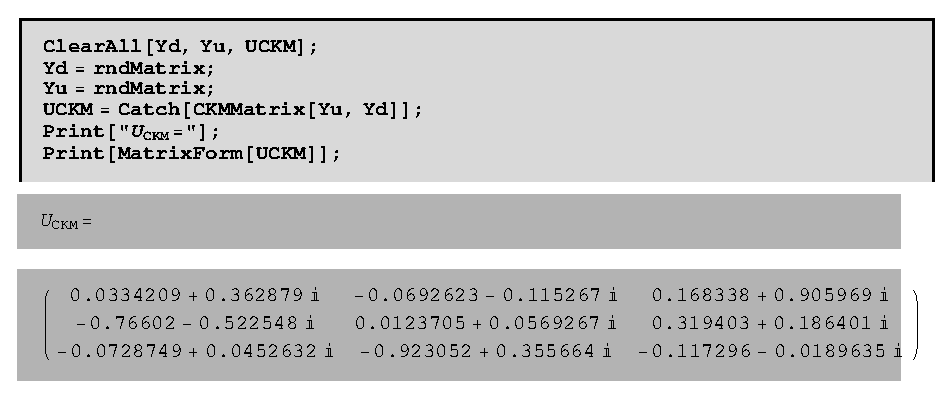
\includegraphics{MPTdoc4.eps}
\end{center}
{\it 
OK, this is a $3\times3$ matrix. Fine. But suppose we're interested in the
Cabbibo angle. Let us try}
\begin{center}
\includegraphics{MPTdoc5.eps}
\end{center}
{\it 
This looks better. According to the above short description, the first list
contains the three angles and the Dirac phase, and the first entry of
the first list is the Cabbibo angle. Let's see\dots }
\begin{center}
\includegraphics{MPTdoc6.eps}
\end{center}
{\it 
All right, our texture is probably only semi-realistic.}

{\it Maybe we are more lucky with neutrinos.}
\begin{center}
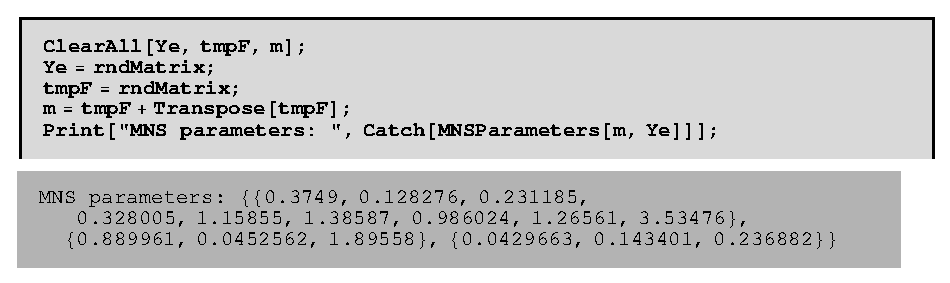
\includegraphics{MPTdoc7.eps}
\end{center}
{\it 
Now a strange thing happened. The entries of the second list, the neutrino mass
eigenvalues, are not ordered ascendingly. This is because it always given in a
form in which it is easy to compare with experiments (cf.\
Sec.~\ref{sec:RemarksMNS}).}

{\it We could be especially interested in the solar mixing angle:}
\begin{center}
\includegraphics{MPTdoc8.eps}
\end{center}
{\it 
Well, also not too close to the central experimental value. Let's try another
texture\dots }

At this point, we decide to leave the `quick start' section, and turn to the
description of the functions.

\clearpage

\section{Description of the functions}
%\enlargethispage{1cm}

\subsection*{\function{MNSMatrix}}
\addcontentsline{toc}{subsection}{\function{MNSMatrix}}

\function{MNSMatrix[$m,Y_e$]} returns the MNS matrix, i.e.\ the matrix
$U_\mathrm{MNS}$ which diagonalizes the (neutrino mass) matrix $m$ in the basis
where the (charged lepton Yukawa coupling) matrix $Y_e$ is diagonal. By
convention, the parameters of $U_\mathrm{MNS}$ fulfill
$0\le\theta_{12}\le\pi/4$, $0\le\theta_{13},\theta_{23}\le \pi/2$ and all  other
parameters range from 0 to $2\pi$. It is possible to fix the hierarchy to be
normal or inverted by calling \function{MNSMatrix[$m,Y_e$,``n'']} or
\function{MNSMatrix[$m,Y_e$,``i'']}, respectively. This option is useful if the
hierarchy changes due to RG evolution. Note that the input matrices
$m$ and $Y_e$ must be numeric.

\subsection*{\function{MNSParameters}}
\addcontentsline{toc}{subsection}{\function{MNSParameters}}

\function{MNSParameters[$m,Y_e$]} returns the MNS mixing and mass parameters
$\{\{\theta_{12},\theta_{13},\theta_{23},\delta,$ $\delta_e,\delta_\mu,\delta_\tau,
\varphi_1,\varphi_2\},\{m_1,m_2,m_3\},\{y_e,y_\mu,y_\tau\}\}$
for a Majorana neutrino matrix $m$ and a Yukawa coupling matrix $Y_e$. The
returned parameters obey the conventions $0\le\theta_{12}\le\pi/4$,
$0\le\theta_{13},\theta_{23}\le \pi/2$ and all other parameters range from 0 to
$2\pi$. It is possible to fix the hierarchy to be
normal or inverted by calling \function{MNSMatrix[$m,Y_e$,``n'']} or
\function{MNSMatrix[$m,Y_e$,``i'']}, respectively. Note that the input matrices $m$ and
$Y_e$ must be numeric. Furthermore, if parameters are undefined, some viable
choice is returned. For instance, if $\theta_{13}=0$, the function returns
$\delta=0$.


\subsection*{\function{DiracMNSMatrix}}
\addcontentsline{toc}{subsection}{\function{DiracMNSMatrix}}

\function{DiracMNSMatrix[$Y_\nu,Y_e$]} returns the MNS matrix for Dirac
neutrinos with Yukawa coupling $Y_\nu$. 

\subsection*{\function{DiracMNSParameters}}
\addcontentsline{toc}{subsection}{\function{DiracMNSParameters}}
 
\function{DiracMNSParameters[$Y_\nu,Y_e$]} returns the MNS mixing parameters 
$\{\theta_{12},\theta_{13},\theta_{23},\delta\}$, $\{y_1,y_2,y_3\}$  (with
$y_i=m_i/v$) and $\{y_e,y_\mu,y_\tau\}$ for neutrino and charged lepton Yukawa
matrices $Y_\nu$ and $Y_e$. Note that these parameters are not sufficient to
determine the unitary matrix which diagonalizes $Y_\nu^\dagger Y_\nu$ in the
basis where  $Y_e^\dagger Y_e$ is diagonal. The additional parameters, required
to reconstruct $U_\mathrm{MNS}^\mathrm{Dirac}$, are unphysical. Note that the
input matrices $Y_\nu$ and $Y_e$ must be numeric. Furthermore, if parameters are
undefined, some viable choice is returned. For instance, if $\theta_{13}=0$, the
function returns $\delta=0$.

\subsection*{\function{CKMMatrix}}
\addcontentsline{toc}{subsection}{\function{CKMMatrix}}

\function{CKMMatrix[$Y_u,Y_d$]} returns the CKM matrix, i.e.\ the matrix
$U_\mathrm{CKM}$ which diagonalizes the (down-type quark Yukawa) matrix $Y_d$ 
in the basis where the (up-type quark Yukawa) matrix $Y_u$ is diagonal. 
Note that the input matrices $Y_u$ and $Y_d$ must be numeric. 


\subsection*{\function{CKMParameters}}
\addcontentsline{toc}{subsection}{\function{CKMParameters}}

\function{CKMParameters[$Y_u,Y_d$]} returns the CKM mixing parameters 
$\{\theta_{12},\theta_{13},\theta_{23},\delta\}$, as well as the Yukawa 
couplings $\{y_u,y_c,y_t\}$ and $\{y_d,y_s,y_b\}$,  for up- and down-type Yukawa
matrices $Y_u$ and $Y_d$. Note that these parameters are not sufficient to
determine the unitary matrix which diagonalizes $Y_d^\dagger Y_d$ in the basis 
where $Y_u^\dagger Y_u$ is diagonal. The additional parameters, required to
reconstruct $U_\mathrm{CKM}$, are unphysical.  Note that the input matrices
$Y_u$ and $Y_d$ must be numeric. Furthermore, if parameters are undefined, some
viable choice is returned. For instance, if $\theta_{13}=0$, the function
returns $\delta=0$.

\section{Remarks}

\subsection{Remarks on the calculation of the CKM matrix}

The input parameters are the Yukawa couplings $Y=(Y_{fg})$ ($Y_u$ and $Y_d$) 
which are defined via the Lagrangean
\begin{equation}
 \mathscr{L}_\mathrm{Yukawa}
 \,=\,
 \overline{\psi_\mathrm{R}^f}\,Y_{fg}\,\psi_\mathrm{L}^g
 +\text{h.c.}\;,
\end{equation}
with R and L indicating right- and left-chiral fields, respectively.  $Y$ can
always be diagonalized by a bi-unitary transformation
\begin{subequations}
\begin{eqnarray}
 \psi_\mathrm{R} & \to & U_\mathrm{R}^\dagger\,\psi_\mathrm{R}\;,\\
 \psi_\mathrm{L} & \to & U_\mathrm{L}^\dagger\,\psi_\mathrm{L}\;,\\
 Y & \to & 
 U_\mathrm{R}^\dagger\,Y\,U_\mathrm{L}
 \,=\,
 \diag(y_1,y_2,y_3)\;,
 \end{eqnarray}
\end{subequations}
with $y_1\le y_2\le y_3$ being the `eigenvalues' of $Y$. Here, $U_\mathrm{L}$
and $U_\mathrm{R}$ are defined (or: can be computed) via
\begin{subequations}
\begin{eqnarray}
 U_\mathrm{L}^\dagger\,Y^\dagger\,Y\,U_\mathrm{L}
 & \stackrel{!}{=} & 
 \diag \left(|y_1|^2,|y_2|^2,|y_3|^2\right)\;,\\
 U_\mathrm{R}^\dagger\,Y\,Y^\dagger\,U_\mathrm{R}
 & \stackrel{!}{=} & 
 \diag \left(|y_1|^2,|y_2|^2,|y_3|^2\right)\;,
\end{eqnarray}
\end{subequations}
respectively. For most applications, $U_\mathrm{R}$ is irrelevant. 

The CKM matrix is calculated as follows:
\begin{enumerate}
 \item Switch to the basis where $Y_u$ is diagonal, i.e.
 \begin{subequations}
 \begin{eqnarray}
  Y_u & \to & (U_\mathrm{R}^{(u)})^\dagger\,Y_u\,U_\mathrm{L}^{(u)}
  \,=\,\diag(y_u,y_c,y_t)\;,\\
  Y_d & \to & (U_\mathrm{R}^{(u)})^\dagger\,Y_d\,U_\mathrm{L}^{(u)}
  \,=:\, Y_d'\;.
 \end{eqnarray}
 \end{subequations}
 \item Calculate $U_\mathrm{L}$ for $Y_d'$. This is $U_\mathrm{CKM}$.
\end{enumerate}

\subsection{Remarks on the calculation of the MNS matrix}
\label{sec:RemarksMNS}

For the MNS matrix, switch to the basis where $Y_e$ is diagonal,
\begin{subequations}
\begin{eqnarray}
 Y_e & \to & U_\mathrm{R}^\dagger\,Y_e\,U_\mathrm{L} 
 \,=\,\diag(y_e,y_\mu,y_\tau)\;,\\
 m_\nu & \to & U_\mathrm{L}^T\,m_\nu\,U_\mathrm{L}
 \,=:\,m_\nu'\;.
\end{eqnarray}
\end{subequations} 
The MNS matrix has to fulfill
\begin{equation}
 U_\mathrm{MNS}^T\,m_\nu'\,U_\mathrm{MNS}
 \,=\,
 \diag(m_1,m_2,m_3)\;,
\end{equation}
where the $m_i$ are real and positive. However, this does not fix
$U_\mathrm{MNS}$ entirely. First of all, there is the obvious ambiguity of
ordering the mass eigenvalues $m_i$. In order to obtain a mixing matrix which
can be compared with the experimental data,  the choice of the prescription is
somewhat subtle. From experiment we know that there is a small mass difference,
called $\Delta m^2_\mathrm{sol}=m_i^2-m_j^2$, and a larger one, referred to as 
$\Delta m^2_\mathrm{atm}=m_k^2 - m_\ell^2$. By convention, the masses are
labeled such that $i,j\ne 3$ while either $k$ or $\ell$ equals 3.  The mass
label 2 is attached to the eigenvector with the lower modulus of the first
component. We are doing this since we want to read off a mixing angle
$\theta_{12}$ less than $45^\circ$. If it then turns out that $m_1>m_2$, the
corresponding mass matrix is most likely not physical.


\subsection{Definition and Extraction of Mixing Parameters}
\label{app:MixingParameters}

\subsubsection{Standard Parametrization}
In this section we describe our conventions and how mixing angles and 
phases can be extracted from mass matrices.
For a general unitary matrix we choose the so-called 
standard parametrization
\begin{eqnarray}\label{eq:StandardParametrizationU}
 U & = &\diag(e^{\I\delta_{e}},e^{\I\delta_{\mu}},e^{\I\delta_{\tau}}) \cdot V \cdot 
 \diag(e^{-\I\varphi_1/2},e^{-\I\varphi_2/2},1)
 \,=:\,
 K_\delta\cdot V\cdot K_\varphi\;,
\end{eqnarray}
where 
\begin{equation}
 V=\left(
 \begin{array}{ccc}
 c_{12}c_{13} & s_{12}c_{13} & s_{13}e^{-\I\delta}\\
 -c_{23}s_{12}-s_{23}s_{13}c_{12}e^{\I\delta} &
 c_{23}c_{12}-s_{23}s_{13}s_{12}e^{\I\delta} & s_{23}c_{13}\\
 s_{23}s_{12}-c_{23}s_{13}c_{12}e^{\I\delta} &
 -s_{23}c_{12}-c_{23}s_{13}s_{12}e^{\I\delta} & c_{23}c_{13}
 \end{array}
 \right)
\end{equation}
with $c_{ij}$ and $s_{ij}$ defined as $\cos\theta_{ij}$ and
$\sin\theta_{ij}$, respectively. 


\subsubsection{Extracting Mixing Angles and Phases}
\label{sec:ExtractingMixingAngles}

In the standard parametrization, the mixing angles $\theta_{13}$ 
and $\theta_{23}$ can be chosen to lie between $0$ and $\frac{\pi}{2}$,
and in the lepton sector by reordering the masses, $\theta_{12}$ can be restricted to $0\le\theta_{12}\le\frac{\pi}{4}$.
For the phases the range between $0$ and $2\pi$ is required.
In order to read off the mixing parameters in the generic case, i.e.\ for none
of the angles $\theta_{ij}$ equal to 0 or $\pi/2$, we use the following
procedure:
\begin{enumerate}
 \item $\theta_{13}=\arcsin(|U_{13}|)$.
 \item $\displaystyle \theta_{12}=\left\{\begin{array}{ll}
 \displaystyle \arctan\left(\frac{|U_{12}|}{|U_{11}|}\right) \quad
        & \text{if}\;U_{11}\ne0\\
 \frac{\pi}{2} & \text{else}
 \end{array}\right.$
 \item $\displaystyle \theta_{23}=\left\{\begin{array}{ll}
 \displaystyle \arctan\left(\frac{|U_{23}|}{|U_{33}|}\right) \quad
        & \text{if}\;U_{33}\ne0\\
 \frac{\pi}{2} & \text{else}
 \end{array}\right.$
 \item $\delta_\mu = \arg(U_{23})$
 \item $\delta_\tau = \arg(U_{33})$
 \item \label{step6}$\displaystyle\delta=
 -\arg\left(\frac{\displaystyle\frac{U_{11}^*U_{13}U_{31}U_{33}^*}
        {c_{12}\,c_{13}^2\,c_{23}\,s_{13}}
        +c_{12}\,c_{23}\,s_{13}}
        {s_{12}\,s_{23}}\right)$\\
 where $i,j\in\{1,2,3\}$ and $i\ne j$.
 \item $\delta_e=\arg(e^{\I\delta}\,U_{13})$
 \item $\displaystyle\varphi_1=2\arg(e^{\I\delta_e}\,U_{11}^*)$
 \item \label{step9}$\displaystyle\varphi_2=2\arg(e^{\I\delta_e}\,U_{12}^*)$
\end{enumerate}
Here we used the relation\footnote{There was an error in an earlier version of
this relation. We are grateful to Yang Bai for pointing it out to us.}
\begin{eqnarray}
 U_{11}^*U_{13}U_{31}U_{33}^*
 & = &
 c_{12}\,c_{13}^2\, 
 c_{23}\,s_{13}
 \left(e^{-\I\delta}\,s_{12}\,s_{23} - c_{12}\,c_{23}\,s_{13}\right)
 \;.\nonumber
\end{eqnarray}
%which holds for $i,j\in\{1,2,3\}$ and $i\ne j$.
Note that this relation is often used in order to introduce 
the Jarlskog invariants %\cite{Jarlskog:1985ht}
\begin{eqnarray}
 J_\mathrm{CP} 
 & = &
 \frac{1}{2} \left| \im (U_{11}^*U_{12}U_{21}U_{22}^*)\right|
 \,=\, 
 \frac{1}{2} \left| \im (U_{11}^*U_{13}U_{31}U_{33}^*)\right|
 \nonumber\\
 & =  &
 \frac{1}{2} \left| \im (U_{22}^*U_{23}U_{32}U_{33}^*)\right|
 \, = \,
 \frac{1}{2}\left|c_{12}\,c_{13}^2\,
    c_{23}\,\sin \delta \,
    s_{12}\,s_{13}\,
    s_{23}\right|\;.
\end{eqnarray}
For the sake of a better numerical stability, one can choose any of the three
combinations. In particular, if the modulus of one of the $U_{ij}$ is very
small, it turns out to be more accurate to choose a combination in which this
specific $U_{ij}$ does not appear.

\subsection{Remarks on special (degenerate) cases}
\label{sec:SpecialCases}

There are several cases where the mixing parameters are not uniquely defined,
e.g.\ when the eigenvalues are degenerate. The package tries to return one set
of possible mixing parameters then.  In some cases, this is not successful, and
an error message is produced. We keep on improving on these cases. Let us,
however, stress that for phenomenologically viable mass matrices, and moderate
deformations thereof, our functions work without problems.
% \subsubsection{Diagonal mass matrices}
% 
% If $Y_e$ and $m_\nu$ are diagonal, the phases are mathematically not
% well-defined. However, even though one may trade $\delta_e$ for $\varphi_1$,
% none of the phases is physical. Hence, \function{MNSParameters} returns only
% non-zero $\delta_e$, $\delta_\mu$ and $\delta_\tau$ in this case.\footnote{For
% the quark sector, i.e.\ \function{CKMParameters}, a similar thing is not
% implemented at the moment\dots}
% 
% \subsubsection{Degenerate masses}
% 
% In the case of degenerate masses, mixings are undefinded, because by definition
% mixings only occur between mass eigenstates which are not fixed in this case.
% \function{MNSParameters} will return arbitrary mixing angles and print a
% warning.
% 
% \subsubsection[$\theta_{13}=0$]{$\boldsymbol{\theta_{13}=0}$}
% \fbox{\parbox{0.9\textwidth}{
% For a zero CHOOZ angle, the Dirac phase is undefined.  Besides, the
% determination of $\varphi_2$ and $\delta_e$ has to be modified.  In
% general, we use
% \begin{subequations} \label{eq:ReadingOffT13Zero}
% \begin{eqnarray}
%         \delta &=& 0 \;, \\
%         \varphi_2 &=& 2 \arg(e^{\I\delta_\mu} U_{22}^*) \;, \\
%         \delta_e &=& \arg(e^{\I\frac{\varphi_2}{2}} U_{12}) \;.
% \end{eqnarray}
% \end{subequations}
% For special values of $\theta_{12}$ and $\theta_{23}$, we apply the
% following modifications:
% \begin{description}
% \item[$\theta_{12}=0$:]
%  \begin{subequations}
%  \begin{eqnarray}
%         \varphi_1 &=& 0 \;, \\
%         \delta_e &=& \arg(U_{11}) \;.
%  \end{eqnarray}
%  \end{subequations}
% \item[$\theta_{12}=\pi/2$:]
%  This case is not considered, as $\theta_{12}$ lies between 0 and
%  $\pi/4$ by definition.  \emph{Ist das richtig?}
% \item[$\theta_{23}=0$:]
%  The phases $\delta_e$, $\delta_\mu$, $\varphi_1$ and $\varphi_2$ are
%  linearly dependent due to the orthonormality of $U$ (cf.\ the case
%  $\theta_{13}=\pi/2$ below), so that we can choose one of them to be
%  zero.
%  \begin{subequations}
%  \begin{eqnarray}
%         \varphi_1 &=& 0 \;, \\
%         \delta_e &=& \arg(U_{11}) \;, \\
%         \varphi_2 &=& 2 \arg(e^{\I\delta_e} U_{12}^*) \;, \\
%         \delta_\mu &=& \arg(-U_{21}) \;.
%  \end{eqnarray}
%  \end{subequations}
% \item[$\theta_{23}=\pi/2$:]
%  \begin{subequations}
%  \begin{eqnarray}
%         \varphi_1 &=& 0 \;, \\
%         \delta_e &=& \arg(U_{11}) \;, \\
%         \varphi_2 &=& 2 \arg(e^{\I\delta_e} U_{12}^*) \;, \\
%         \delta_\tau &=& \arg(-e^{\I\frac{\varphi_2}{2}} U_{32}) \;.
%  \end{eqnarray}
%  \end{subequations}
% \end{description}
% }}
% 
% 
% \subsubsection[$\theta_{13}=\pi/2$]{$\boldsymbol{\theta_{13}=\pi/2}$}
% \fbox{\parbox{0.9\textwidth}{
% This case often occurs when the neutrino mass hierarchy changes, i.e.\
% $\Delta m^2_\mathrm{sol}$ overtakes $\Delta m^2_\mathrm{atm}$ during the
% running.  As the rows and columns of the mixing matrix have to be
% normalized, it can be written as
% \begin{equation} \label{eq:T13Pi2Int}
%         U =
%         \begin{pmatrix}
%         0 & 0 & e^{\I\delta_1} \\
%         -e^{\I\varphi_{21}} \sin\theta & e^{\I\varphi_{22}} \cos\theta & 0\\
%         -e^{\I\varphi_{31}} \cos\theta &-e^{\I\varphi_{32}} \sin\theta & 0\\
%         \end{pmatrix} ,
% \end{equation}
% where the positions of $\sin$ and $\cos$ and of the minus signs are
% arbitrary, of course.  We choose the angle $\theta$ to equal
% $\theta_{23}$ and the phase of the 13-element to equal $\delta_e$.  This
% implies $\theta_{12}=0$ and $\delta=0$.  Furthermore, from the
% orthogonality of the rows we find
% $U_{21}^* U_{22} + U_{31}^* U_{32} = 0$, which means that
% $\varphi_{21}-\varphi_{22}-\varphi_{31}+\varphi_{32} = n \, 2\pi$
% ($n\in\mathbbm{Z}$).  Consequently, one of the remaining four phases is
% arbitrary, and we choose $\varphi_1=0$.  Comparing
% eq.~\eqref{eq:T13Pi2Int} to the standard parametrization now leads to
% the parametrization of the MNS matrix for $\theta_{13}=\pi/2$,
% \begin{equation} \label{eq:MNSParametrizationT13Pi2}
%         U =
%         \begin{pmatrix}
%         0 & 0 & e^{\I\delta_e} \\
%         -e^{\I\delta_\mu} s_{23} & e^{\I(\delta_\mu-\varphi_2/2)}\,c_{23} & 0\\
%         -e^{\I\delta_\tau} c_{23} &-e^{\I(\delta_\tau-\varphi_2/2)} s_{23} & 0\\
%         \end{pmatrix} .
% \end{equation}
% Thus, the mixing parameters are determined as follows:
% \begin{subequations} \label{eq:ReadingOffT13Pi2}
% \begin{eqnarray}
%    \delta & = & 0\;,\\
%    \delta_e & = & \arg (U_{13})\;,\\
%    \theta_{12} & = & 0\;,\\
%    \theta_{23} & = & \arctan (|U_{21}/U_{31}|)\;,\\
%    \varphi_1 & = & 0\;,\\
%    \delta_\mu & = & \arg(-U_{21})\;,\\
%    \varphi_2 & = & 2\,(\delta_\mu - \arg(U_{22}))\;,\\
%    \delta_\tau & = & \arg(-U_{31})\;.
% \end{eqnarray}
% \end{subequations}
% For $U_{21}=0$ ($\theta_{23}=0$), we use $\delta_\mu = \arg(U_{22})$,
% $\varphi_2 = 0$.  For $U_{31}=0$ ($\theta_{23}=\pi/2$), we can also set
% $\varphi_2=0$; the phase $\delta_\tau$ is then determined from
% $\delta_\tau = \arg(-U_{32})$.
% \\ This also affects functions based on \function{MPT3x3MixingParameters[$U$]},
% such as \function{MNSParameters} and \function{CKMParameters}.
% \dots\emph{under construction}\dots 
% \emph{Ist dieser Kommentar noch aktuell? (J.)}
% }}
% 
% 

\section{Trouble-Shooting}

There may be bugs in the software. We will collect them on the web page 
\begin{center}
\url{http://www.ph.tum.de/~rge/MPT/bugs.html}\;. 
\end{center}
In case you encounter a new bug, or if you have other
suggestions, please write an email to \texttt{rge@ph.tum.de}.

\clearpage
\appendix
\section{Theorems on Matrix-Diagonalization}
\subsection*{Hermitean Matrices}
\begin{Theorem}
 Hermitean matrices $M$ can be diagonalized by unitary transformations,
 \begin{equation}
        U^\dagger M U = \diag(M_1,\dots,M_n) \;,
 \end{equation}
 where $U$ is unitary and the eigenvalues $M_i$ are real. The columns of
 $U$ contain the eigenvectors of $M$.
\end{Theorem}
\begin{Proof}
 See the standard textbooks on linear algebra.
\end{Proof}

\subsection*{General Matrices (Biunitary Diagonalization)}
\begin{Theorem} \label{th:BiunitaryDiag}
 A general, non-singular matrix $M$ can be diagonalized by a 
 \emph{biunitary} transformation\index{biunitary},
 \begin{equation} \label{eq:BiunitaryDiag}
        U_\mathrm{L}^\dagger M U_\mathrm{R} = \diag(M_1,\dots,M_n) \;,
 \end{equation}
 if none of the eigenvalues of $M^\dagger M$ equals zero.
 $U_\mathrm{L}$ and $U_\mathrm{R}$ are unitary, and $M_i$ are real and
 positive.
 The matrices $U_\mathrm{L}$ and $U_\mathrm{R}$ can be found by
 determining the unitary transformations which diagonalize $M M^\dagger$
 and $M^\dagger M$, respectively, i.e.\
 \begin{subequations}
 \begin{eqnarray}
        U_\mathrm{L}^\dagger \, M M^\dagger \, U_\mathrm{L} &=&
         \diag(M_1^2,\dots,M_n^2) \;,
 \\
        U_\mathrm{R}^\dagger \, M^\dagger M \, U_\mathrm{R} &=&
         \diag(M_1^2,\dots,M_n^2) \;.
        \label{eq:DefUR}
 \end{eqnarray}
 \end{subequations}
\end{Theorem}
\begin{Proof}
 Define
 \begin{equation}\label{eq:Mohapatra4.75}
        H^2 := M M^\dagger \;,
 \end{equation}
 which is obviously Hermitean and can therefore be diagonalized by a
 unitary transformation,
 \begin{equation}
        U_\mathrm{L}^\dagger \, M M^\dagger \, U_\mathrm{L} =
         \diag(M_1^2,\dots,M_n^2) =: D^2 \;,
 \end{equation}
 where $M_i$ are real and positive.
 Define $D$ as the diagonal matrix containing the square-roots of $D^2$.
 Then obviously
 \begin{equation} \label{eq:DefH}
        H := U_\mathrm{L} D U_\mathrm{L}^\dagger 
 \end{equation}
 satisfies \fref{eq:Mohapatra4.75}. With $V:=H^{-1}M$, 
 which is unitary because
 \begin{equation}
        V^\dagger V \stackrel{H^\dagger=H}{=}
        M^\dagger H^{-1} H^{-1} M \stackrel{\eqref{eq:Mohapatra4.75}}{=}
        M^\dagger (M M^\dagger)^{-1} M = \mathbbm{1} \;,
 \end{equation}
 we find
 \begin{equation} \label{eq:ProofCompl}
        M = H V \stackrel{\eqref{eq:DefH}}{=}
        U_\mathrm{L} D U_\mathrm{R}^\dagger \;,
 \end{equation}
 where $U_\mathrm{R} := V^\dagger U_\mathrm{L}$ is unitary, so that
 \fref{eq:BiunitaryDiag} is proven. Furthermore, $U_\mathrm{R}$
 diagonalizes $M^\dagger M$, since
 \begin{equation}
        U_\mathrm{R}^\dagger M^\dagger M U_\mathrm{R}
        \stackrel{\eqref{eq:ProofCompl}}{=}
        U_\mathrm{R}^\dagger \, U_\mathrm{R} D U_\mathrm{L}^\dagger \,
         U_\mathrm{L} D U_\mathrm{R}^\dagger \, U_\mathrm{R} = D^2 \;,
 \end{equation}
 which proves \fref{eq:DefUR}.
\end{Proof}

\subsection*{Symmetric Matrices}
\begin{Theorem} \label{th:SymmetricMatrixDiag}
 Complex symmetric matrices can be diagonalized by a unitary matrix $U$,
 \begin{equation}
        U^T M U = \diag(M_1,\dots,M_n) := D \;,
 \end{equation}
 where
 \begin{equation}
        U^\dagger \, M^\dagger M \, U = D^2 \;,
 \end{equation}
 i.e.\ the real numbers $M_i$ are the square roots of the eigenvalues of
 $M^\dagger M$.
\end{Theorem}
\begin{Proof}
 From theorem \ref{th:BiunitaryDiag} we know that 
 \begin{equation}
        M = U_\mathrm{L} D U_\mathrm{R}^\dagger \;,
 \end{equation}
 where $U_\mathrm{L}$, $U_\mathrm{R}$ and $D$ are uniquely 
 determined.\footnote{Note that $U_\mathrm{L}$, $U_\mathrm{R}$ are
 not always unique: If the eigenvalues
 of $D$ are degenerate, there exist matrices $U$ which diagonalize
 $M^\dagger M$, i.e. $U^\dagger\,M^\dagger M\, U=D$, which however
 do not diagonalize $M$. In this case, $M$ can still be diagonalized,
 but the matrix which does the job can not simply be obtained by calculating
 the eigenvectors of $M^\dagger M$.}
 As $M$ is symmetric, it follows that
 \begin{equation}
        M = M^T = U_\mathrm{R}^* D U_\mathrm{L}^T \;.
 \end{equation}
 On the other hand, we can view the last equation as the diagonalization
 of $M^T$, which is uniquely determined as well according to theorem
 \ref{th:BiunitaryDiag}.  Hence, we conclude 
 $U_\mathrm{L}=U_\mathrm{R}^*$, which completes the proof if we set
 $U:=U_\mathrm{R}$ and take into account \fref{eq:DefUR}.
\end{Proof}

% \section{Some thoughts during implementation}
% 
% \subsection*{$\theta_{13}$ problem}
% 
% if $\theta_{13}=\pi/2$ is encountered. there are `angle and phase moduli', i.e.\
% combinations of angles and phases which do not change the resulting unitary
% matrix when plugged in. This is obvious since the only non-trivial information
% is encoded in the bottom-left $2\times2$ sub-block (and the phase of $U_{13}$).
% This sub-block can be parametrized by one angle.
% 
% \subsection*{degenerate eigenvalues}
% 
% Mathematica has the function \function{SingularValueDecomposition[$m$]} which
% returns three matrices $U$, $V$ and $W$ such that $W$ is diagonal, $U$ and
% $V$ are unitary and 
% \begin{equation}\label{eq:SingularValueDecomposition}
%  m\,=\,U\,W\,V^\dagger\;.
% \end{equation} 
% \begin{itemize}
%  \item This function is obviously very  useful for matrix diagonalization (it almost
% does everything we need). 
%  \item For non-degenerate eigenvalues and symmetric $m$ we
% have due to \ref{th:SymmetricMatrixDiag} that $U^*=V$.
%  \item However, for degenerate mass eigenvalues,
% \function{SingularValueDecomposition[$m$]} returns still $U$, $V$ and $W$ such
% that \eqref{eq:SingularValueDecomposition} holds, but $U^*\ne V$ in general.
% In this case, one (combination of) mixing angle(s) is unphysical. $U^*$  and $V$
% differ by an unphysical rotation. If one takes the average, one can construct a
% matrix $V$ such that $V^TM\,V$ is diagonal.
%  \item Unfortunately, when trying to identify these unphysical parameters, one
%  runs into the $\theta_{13}=\pi/2$ problem. So, this has to be solved first.
% \end{itemize}
% 
% \bibliography{Running}
% \bibliographystyle{TitleAndArxiv}

\end{document}
